\chapter{El problema del clustering con restricciones}\label{ch:clustering}

El clustering con restricciones es un problema perteneciente al ámbito del aprendizaje semi-supervisado, tal y como se dijo en la introducción. Por ello, es lógico dedicar un apartado que sirva como introducción al aprendizaje semi-supervisdado antres de comenzae a definir y explicar con detalle el clustering con restricciones. Para ello, se ha tomado como referencia principal el capítulo introductorio de \cite{chapelle2006semi}.

\section{Introducción al aprendizaje semi-supervisado}


El aprendizaje semi-supervisado es una de las cuatro modalidades existentes de aprendizaje automático, quizá la menos conocida de ellas. Podría decirse que es un híbrido entre aprendizaje supervisado y aprendizaje no supervisado.

En aprendizaje no supervisado (ver capítulo anterior), se dispone únicamente del conjunto de datos $\textbf{X} = ( \textbf{x}_1, \textbf{x}_2, \dots, \textbf{x}_N )$, compuesto por $N$ muestras o puntos, de forma que el objetivo consiste en encontrar patrones o estructuras en $\textbf{X}$ que puedan ser interesantes. Además del clustering o agrupación, existen otras formas de aprendizaje no supervisado, como la detección de \emph{outliers} o las técnicas de reducción de dimensionalidad.

En aprendizaje supervisado, por su parte, se pretende encontrar una aplicación $\textbf{x} \mapsto y$ dado un conjunto de entrenamiento compuesto por pares $(\textbf{x}_i,y_i)$. En este caso, $y_i$ son las etiquetas de las muestras $\textbf{x}_i$, de forma que, además de $\textbf{X}$, se dispone también del vector de etiquetas $\textbf{y} = (y_1,\dots,y_N)^T$. Nótese que para cada muestra siempre se dispone de una etiqueta. Si las etiquetas adoptan valores continuos ($y_i \in \mathbb{R}$ o $y_i \in \mathbb{R}^p$), la tarea se conoce como regresión, mientras que si adoptan valores discretos (es decir, valores de conjuntos finitos), se conoce como clasificación. Las dos grandes categorías de algoritmos de aprendizaje supervisado son los algoritmos generativos, los cuales pretenden calcular la distribución de problabilidad condicionada $P(\textbf{x}|y)$ para obtener a partir de ella la distribución $P(y|\textbf{x})$, y los algoritmos discriminativos, que en general se limitan a obtener $P(y|\textbf{x})$.

El aprendizaje semi-supervisado es una modalidad a medio camino entre el supervisado y el no supervisado. Efectivamente, se dispone del conjunto de datos sin etiquetas $\textbf{X}$, pero además también se dispone de una cierta cantidad de información supervisada, aunque no para todas las muestras.

En muchas ocasiones, la información supervisada disponible son las etiquetas de algunos puntos de $\textbf{X}$. En tales casos, el conjunto de datos $\textbf{X}$ puede dividirse en dos subconjuntos: por un lado, el conjunto $\textbf{X}_e = (\textbf{x}_0,\dots,\textbf{X}_e)$ para el cual se disponen de las etiquetas $\textbf{y}_e = (y_1,\dots,y_e)$, y por otro lado el conjunto sin etiquetas $\textbf{X}_s = (\textbf{x}_{e+1},\dots,\textbf{X}_{e+s})$.

En otros casos, la información supervisada se da en forma de restricciones. Dichas restricciones indican si algunos ciertos pares de muestras tienen (o no) la misma etiqueta, o si forman parte o no del mismo cluster. A este tipo de aprendizaje semi-supervisado pertenece precisamente el problema que nos ocupa: el clustering con restricciones.

¿Cuándo tiene sentido usar técnicas semi-supervisadas, pudiendo emplear directamente aprendizaje supervisado? En los casos en los que obtener un etiquetado de los datos resulte demasiado costoso, cosa que suele ocurrir a menudo. Por ejemplo: generar conjuntos de datos con grabaciones de voz para un sistema de reconocimiento de voz es una tarea fácil, ya que pueden o bien grabarse expresamente para ello o bien recopilarse de grabaciones previas. Sin embargo, etiquetar ese conjunto de datos con grabaciones no es tan sencillo, pues requiere de alguien que escuche todas esas grabaciones y las transcriba. Otros ejemplos en los que esto también se cumple pueden ser la clasificación de documentos o páginas web, que necesitan que sean leídas por personas, o la clasificación de imágenes, pues igualmente hacen falta personas que vean esas imágenes e indiquen cuál es su contenido.

Dicho esto, ¿podemos esperar un buen rendimiento de las técnicas semi-supervisadas en comparación con las supervisadas? Lo cierto es que sí, pero es necesario asumir algunas hipótesis. Una de ellas, con respecto a la continuidad de la distribución de los datos, consiste en asumir que si dos puntos $\textbf{x}_1$ y $\textbf{x}_2$ en una región con alta densidad de puntos están cerca el uno del otro, entonces sus respectivos valores de salida $y_1$ e $y_2$ también deberían ser cercanos entre ellos. En el caso concreto del clustering, esto se traduce a que, si dos puntos pertenecen a la misma agrupación o cluster (región de alta densidad), entontes lo lógico sería pensar que pertenecen a la misma clase, o que poseen la misma etiqueta. De esta observación se puede inferir que las fronteras de decisión, o sea, los límites entre clusters distintos, deberían transcurrir por regiones de poca densidad, ya que si, de lo contrario, una frontera se situase en una región de alta densidad, un cluster quedaría cortado por dicha frontera. \cite{chapelle2006semi}

\section{Clustering con restricciones}

Esta sección, centrada en describir y formular el problema del clustering con restricciones, tomará como referencia el análisis realizado por Davidson y Basu en \cite{davidson2007survey}.

El clustering con restricciones permite incorporar conocimiento experto sobre el problema en cuestión en forma de restricciones. Existen dos tipos de restricciones a nivel de instancia, definidas por primera vez en \cite{wagstaff2000clustering}:
\begin{itemize}
	\item \textbf{Restricciones \emph{Must-Link}} (ML), denotadas $c_{=}(\textbf{x},\textbf{y})$. Indican que los puntos \textbf{x} e \textbf{y} deben pertenecer a un mismo cluster.
	\item \textbf{Restricciones \emph{Cannot-Link}} (CL), denotadas $c_{\not=}(\textbf{x},\textbf{y})$. Indican que los puntos \textbf{x} e \textbf{y} no pueden pertenecer a un mismo cluster.
\end{itemize}

En particular, las restricciones ML resultan ser una relación de equivalencia entre puntos, por lo que cumplen las propiedades reflexiva, simétrica y transitiva. Esta última es especialmente relevante, ya que permite generar más restricciones ML a partir de las que ya hubiese disponibles:

\begin{observacion}
	\textbf{\emph{Las Restricciones \emph{Must-Link} Son Transitivas.}} Sean $CC_i$ y $CC_j$ componentes conexas, es decir, subgrafos totalmente conectados con restricciones $ML$. Sean $x$ e $y$ dos puntos o instancias en $CC_i$ y $CC_j$ respectivamente. Si $c_{=}(x,y)$ tal que $x \in CC_i,~y \in CC_j$,  entonces $c_{=}(a,b)~\forall a,b: a\in CC_i,~b \in CC_j$ \cite{davidson2007survey} \cite{basu2008constrained}. 
\end{observacion}

Análogamente, aún sin constituir una relación de equivalencia, también pueden inferirse nuevas restricciones CL a partir de otras:

\begin{observacion}
	\textbf{\emph{Las Restricciones \emph{Cannot-Link} Pueden Conllevar Más Restricciones \emph{Cannot-Link} .}} Sean $CC_i$ y $CC_j$ componentes conexas, es decir, subgrafos totalmente conectados con restricciones $ML$. Sean $x$ e $y$ dos puntos o instancias en $CC_i$ y $CC_j$ respectivamente. Si $c_{\not=}(x,y)$ donde $x \in CC_i, y \in CC_j$, entonces $c_{\not=}(a,b)~\forall a,b: a\in CC_i, b \in CC_j$ \cite{davidson2007survey} \cite{basu2008constrained}.
\end{observacion}

Como puede verse, las restricciones ML y CL albergan mucho potencial a pesar de su simpleza. Con ellas es posible encadenar nuevas restricciones, permitiendo aumentar la colección de restricciones de la que se dispone inicialmente.

Además de estas dos propiedades, también existen otras formas de generar nuevas restricciones ML y CL basadas en la distancia:

\begin{itemize}
	\item \textbf{Restricciones Delta} ($\delta$). Para cada punto \textbf{x}, se establece una restricción Must-Link con cada punto \textbf{y} cuya distancia con \textbf{x} sea menor que un cierto valor $\delta$. Con esto, es posible garantizar que los puntos pertenecientes a distintos clusters estén separados por una distancia mayor o igual a $\delta$.
	\item \textbf{Restricciones Épsilon} ($\epsilon$). Para cada punto \textbf{x}, se establece una restricción Must-Link con al menos un punto \textbf{y} cuya distancia con \textbf{x} sea menor o igual a un cierto valor $\epsilon$. Esto permite forzar a que todos los puntos tengan un vecindario de diámetro $\epsilon$.
\end{itemize}

Los métodos que hacen uso de este tipo restricciones que afectan a parejas de instancias (Must-Link, Cannot-Link) se conocen como \textbf{métodos basados en restricciones}. Éstos métodos modifican al algoritmo de clustering en sí para que las restricciones establecidas introduzcan un sesgo en el proceso de búsqueda para poder encontrar la solución correcta. En esencia, existen dos tipos de métodos basados en restricciones:

\begin{figure}
	\centering
	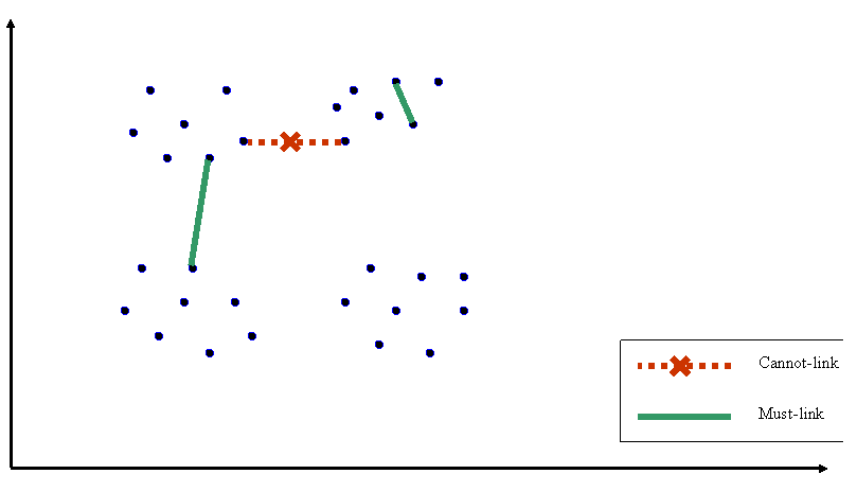
\includegraphics[width=0.75\textwidth]{Images/const_clust}
	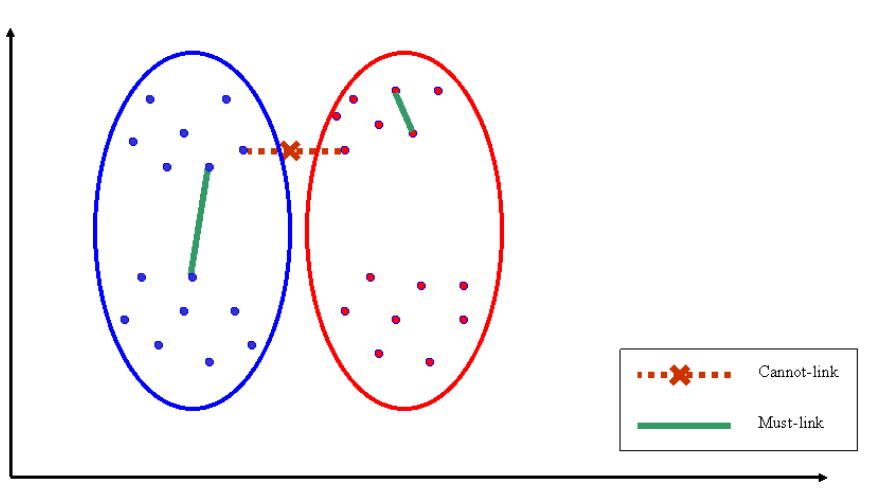
\includegraphics[width=0.75\textwidth]{Images/const_clust_sol}
	\caption[Arriba, un pequeño conjunto de datos con restricciones ML y CL. Abajo, una solución de clustering para ese conjunto de datos que satisface a todas las restricciones.]{Arriba, un pequeño conjunto de datos con restricciones ML y CL. Abajo, una solución de clustering para ese conjunto de datos que satisface a todas las restricciones. \cite{davidson2007survey}}
	\label{fig:const_clust_sol}
\end{figure}


\begin{enumerate}
	\item Aquellos que obligan a que se cumplan las restricciones, de forma que se pretende encontrar la mejor solución que satisfaga a todas ellas \cite{wagstaff2001constrained} \cite{davidson2005hierarchical}.
	\item Aquellos que obligan parcialmente a que se cumplan permitiendo que no todas sean satisfechas, de forma que se busca, por un lado, encontrar la mejor solución de clustering posible, y por otro, maximizar el número de restricciones satisfechas \cite{basu2004active} \cite{segal2003discovering} \cite{davidson2005clustering} \cite{law2005model}.
\end{enumerate}


La otra gran categoría de técnicas de clustering con restricciones está conformada por los llamados \textbf{métodos basados en la distancia}. En ellos, el algoritmo de clustering emplea una medida de distancia \emph{entrenada} o adaptada para que se puedan satisfacer todas las restricciones, en lugar de la distancia euclídea convencional. En este sentido, el espacio es modificado para que se puedan satisfacer las restricciones, de forma que las instancias sujetas a restricciones Must-Link quedan cerca unas de otras, y las restricciones Cannot-Link terminan alejadas entre ellas.

\begin{figure}
	\centering
	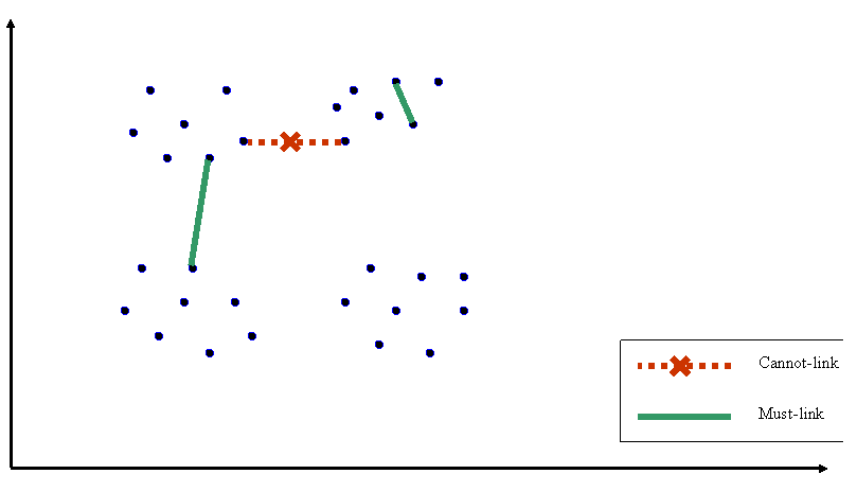
\includegraphics[width=0.75\textwidth]{Images/const_clust}
	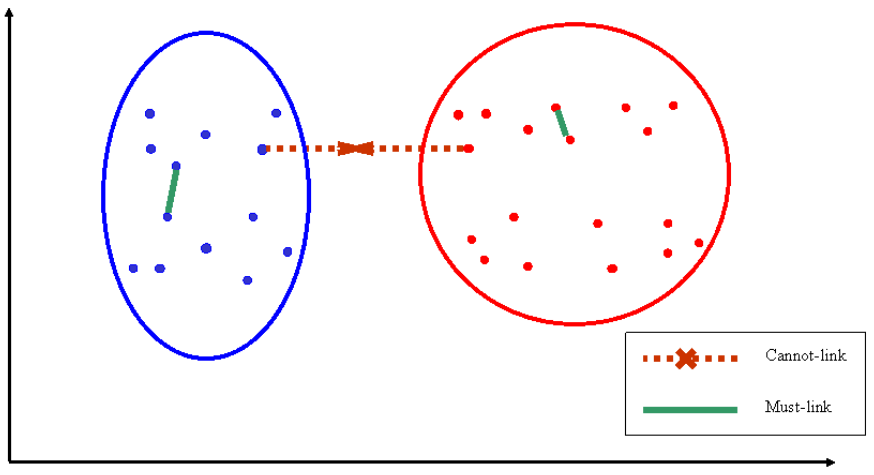
\includegraphics[width=0.75\textwidth]{Images/const_clust_dist}
	\caption[Arriba, un pequeño conjunto de datos con restricciones ML y CL. Abajo, una solución de clustering para ese conjunto de datos después de haber modificado las distancias entre las instancias teniendo en cuenta esas restricciones.]{Arriba, un pequeño conjunto de datos con restricciones ML y CL. Abajo, una solución de clustering para ese conjunto de datos después de haber modificado las distancias entre las instancias teniendo en cuenta esas restricciones. \cite{davidson2007survey}}
	\label{fig:const_clust_dist}
\end{figure}


\subsection{Ventajas e inconvenientes del uso de restricciones en clustering}

Como todo, el clustering con restricciones tiene una serie de beneficios así como de problemas comparado con el clustering básico. En los dos siguientes apartados veremos de cuáles se tratan.

\subsubsection{Ventajas}

Existen dos beneficios principales de la aplicación de restricciones al problema del clustering. La primera, y quizá la más relevante, es la siguiente:

\begin{observacion} 
	\textbf{Las Restricciones Mejoran la Exactitud en el Caso Promedio.} Al hacer el promedio con muchos conjuntos de restricciones distintos, el rendimiento de la predicción de las etiquetas correctas tenderá a aumentar con respecto a no usar restricciones en absoluto. \cite{davidson2007survey}.
	\label{ob:improvement}
\end{observacion}


Se han llevado a cabo numerosos estudios en los que se ha comprobado que esto se cumple. Por poner un ejemplo, en \cite{wagstaff2000clustering} se logró una mejora del 6\%, 10\% y del 20\% para los conjuntos de datos de la UCI Soybean, Pos y Mushroom respectivamente, con tan solo un conjunto de 40 restricciones a nivel de instancia.

El segundo beneficio del uso de restricciones es la posibilidad de \emph{amoldar} la forma geométrica de los clusters resultantes. En \cite{wagstaff2001constrained}, por ejemplo, donde se emplean datos de rutas de coches vía GPS, los clusters que deberían representar las vías no salen con la forma alargada que cabría esperar. Por medio de la implantación de restricciones Cannot-Link entre instancias situadas a más de 4 metros de distancia entre ellas en dirección perpendicular a las carreteras, fue posible corregir los clusters generados para que adoptasen la forma esperada. De esta forma, o con la formación de restricciones $\delta$ y restricciones $\epsilon$, es posible modificar las propiedades geométricas de la forma que mejor convenga.

\subsubsection{Desventajas}

A pesar de haberse demostrado los beneficios del uso de restricciones, existen dos importantes limitaciones que se han de tener en cuenta.

El primer problema es la \textbf{factibilidad}, es decir, el hecho de que sea factible satisfacer todas las restricciones del conjunto de restricciones dado. Si no se emplea un buen método para generar las restricciones, estas pueden contradecirse las unas a las otras, por lo que puede que no exista ninguna solución de clustering que las satisfaga a todas. Por ejemplo, si tenemos dos objetos $\textbf{x}_a$ y $\text{x}_b$, bastaría con definir las restricciones $c_{=}(\textbf{x}_a,\textbf{x}_b)$ y $c_{\not =}(\textbf{x}_a,\textbf{x}_b)$ para tener una contradicción. Una definición más formal de este problema es la siguiente:

\begin{definicion}
 \emph{\textbf{Problema de la factibilidad}:} Dado un conjunto de datos $\textbf{X}$, un conjunto de restricciones $\textbf{R}$, una cota inferior $K_l$ y una cota superior $K_u$, ¿existe una partición de $\textbf{X}$ en $k$ clusters tal que $K_l \leq k \leq K_u$ y que todas las restricciones en $\textbf{R}$ sean satisfechas? \cite{davidson2007survey} \cite{davidson2005clustering}.
\end{definicion}

El problema de la factibilidad es NP-Completo cuando se emplea una conjunción de restricciones Cannot-Link \cite{davidson2007survey}, por lo que el problema de encontrar la mejor solución que satisfaga todas las restricciones puede volverse inviable. Determinar si una única solución satisface todas las restricciones ya es complejo de por sí, pero obtener la mejor solución que las satisfaga a todas lo es aún más.

El otro gran problema del uso de restricciones para el problema del clustering es que \textbf{no todos los conjuntos de restricciones son útiles}, aunque sí sean satisfacibles. Normalmente, se asume que las restricciones son \emph{pistas} que ayudan durante el proceso de búsqueda, puesto que introducen información sobre la solución óptima o verdadera y permiten que, en teoría, sea más fácil obtener una solución similar a la verdadera.

Pensar eso no es descabellado teniendo en cuenta la observación \ref{ob:improvement}. Sin embargo, hay que tener en cuenta que las restricciones mejoran los resultados en el caso promedio, y no todos los conjuntos de restricciones provocarán una mejora. Por ejemplo, en \cite{davidson2006measuring} se demuestra que aún empleando restricciones sin ruido, sin errores y obtenidas directamente de la solución verdadera, es posible que algunos conjuntos de restricciones concretos afecten negativamente al rendimiento. Esto parece ir en contra de lo que suele deducir de otros experimentos, pero el motivo es, de nuevo, que en ellos se promedian los resultados, y en tales casos la observación \ref{ob:improvement} vuelve a cumplirse:

\begin{observacion}
 \emph{\textbf{Conjuntos de Restricciones Concretos Pueden Tener Efectos Adversos}:} Algunos conjuntos de restricciones generados a partir de las etiquetas de la solución verdadera, con la que se evalúan los clusters obtenidos, pueden disminuir la exactitud de la predicción de esas mismas etiquetas \cite{davidson2007survey}.
\end{observacion}


\subsection{Ejemplos de uso}

En \cite{davidson2007survey} se enumeran algunos casos reales de aplicación del clustering con restricciones:
\begin{itemize}
	\item \textbf{Imágenes}: clustering de píxeles para identificación de objetos en la navegación del robot Aibo, mediante el uso de restricciones espaciales (restricciones $\epsilon$ y $\delta$, por ejemplo) [cita]
	\item \textbf{Vídeos}: inclusión de restricciones ML en grupos de píxeles que representan el mismo objeto a lo largo de sucesivos fotogramas [Yan et al. 2004]
	\item \textbf{Biología}: clustering de genes, con restricciones ML para los genes y proteínas que participen en los mismos procesos celulares [Xenarios et al. 2001] [Segal et al. 2003].
	\item \textbf{Audio}: análisis de audio, empleando restricciones para distinguir si dos locutores corresponden a la misma persona o si son diferentes [Bar-Hillel et al. 2003].
	\item \textbf{GPS}: detección de vías y carreteras, empleando restricciones ML en posiciones por las que ha pasado el mismo coche por una carretera, y restricciones CL entre coches situados a más de 4 metros de distancia entre ellas en dirección perpendicular a la de la circulación \cite{wagstaff2001constrained}.
\end{itemize}

